%-*- coding: utf-8 -*-
\subsubsection{Modèle du domaine}
\rowcolors{2}{Turquoise}{} % {1}{red!26!green!29!blue!31!}{}
\begin{figure}
  \centering
      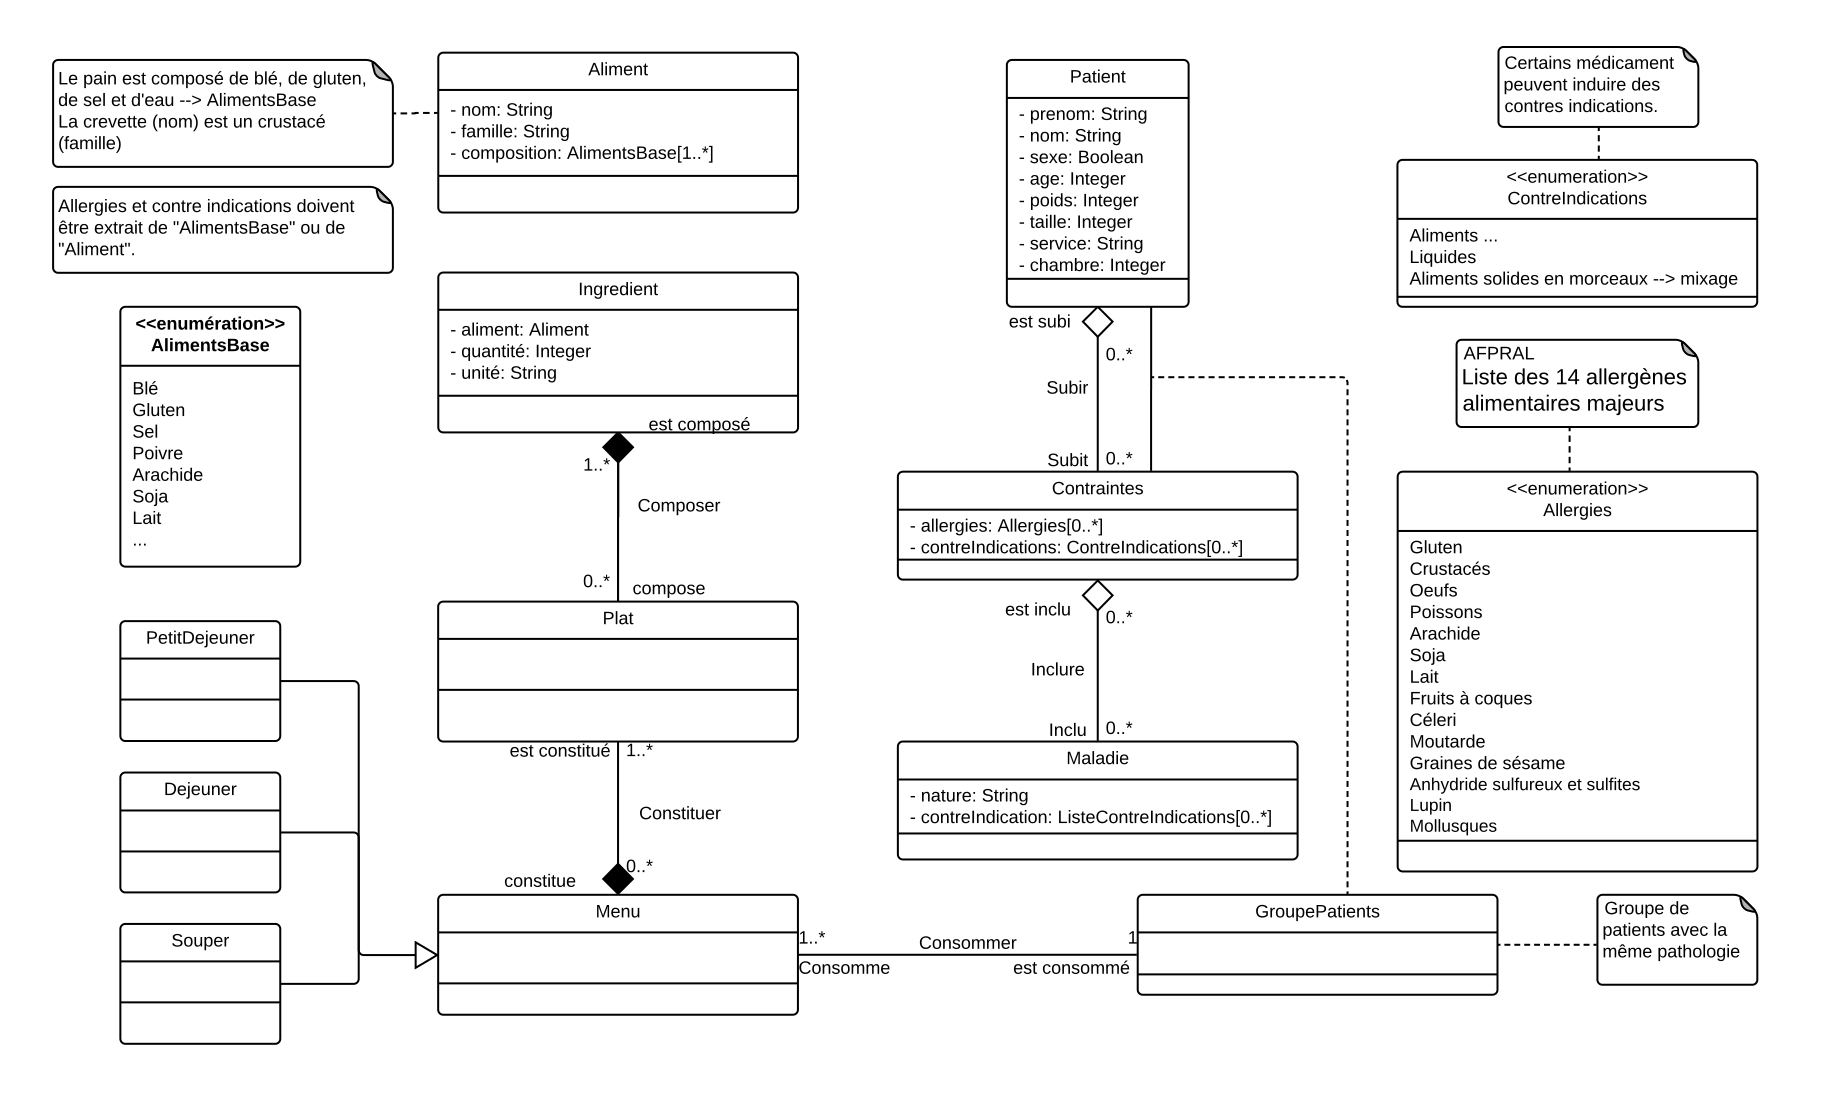
\includegraphics[width=1.00\textwidth]{../../ModeleDuDomaine/ModeleDuDomaine.png} %
\caption{Modèle du domaine}
\label{ModeleDuDomaine}
\end{figure}

\newcommand{\classe}[1]{\emph{\textbf{#1}}}
\newcommand{\attribut}[1]{\emph{#1}}
\newcommand{\regleD}[1]{\textcolor{NavyBlue}{#1}}
\newcommand{\regleT}[1]{\textcolor{ForestGreen}{#1}}

Le modèle du domaine est représenté \autoref{ModeleDuDomaine}. Ce projet ayant pour objet l'alimentation des personnes hospitalisées, nous considérons les pathologies de ces personnes sous l'aspect de leur impact sur le plan alimentaire, et pour être plus précis sur les aliments qui s'avéreraient être interdits à cause de telle ou telle pathologie. Ces pathologies constituant des contraintes sur le plan alimentaire, c'est la classe \classe{Contrainte} qui les décrit. Elle a un attribut \attribut{nom} pour la désigner, un attribut \attribut{type} pour savoir sur quel type d'attribut aliment porte la contrainte (forme, famille, texture, aliment de base), un attribut \attribut{nature} qui permet de déterminer s'il sagit d'une allergie\footnote{\label{allergies}\href{https://allergies.afpral.fr/allergie/en-savoir-plus-sur-les-allergies/alimentaires/89-liste-des-14-allergenes-alimentaires-majeurs}{AFPRAL: Liste des 14 allergènes alimentaires majeurs}}, d'une contre~indications\footnote{\label{contreIndications}La prise de certains médicaments interdit la consommation de certains aliments.} ou d'une maladie. Elle a aussi une collection d'instance de la classe \classe{Ingredient} en attribut; qui porte dans un de ses attributs (désigné par la valeur de l'attribut \attribut{type} de la classe \classe{Contrainte}) l'objet de la contrainte. La classe \classe{GroupePatients} permet d'avoir la liste des patients qui subissent les mêmes contraintes alimentaires.

Les aliments étant à la base de la composition des plats constituant les menus, c'est la classe \classe{Ingrédient} qui les décrit. Les noms des attributs de cette classe parlent d'eux même; nous allons cependant expliquer l'attribut \attribut{texture} qui est un terme métier pour dire si l'on travaille avec des \href{http://plone.vermeil.org:8080/ehpad/Bibliotheque/Memoires/annee-2012-2013/07 - Les textures modifiees et le plaisir de manger de Jacques Caby.pdf}{aliments à texture modifiée} (mixés) ou à texture maintenue (entiers). Cette classe définit l'ensemble des aliments qu'ils soient de base (le blé, l'eau le sel) ou non (le pain). L'attribut \attribut{alimentDeBase} indique que l'on a à faire à un aliment de base (lorsqu'il est vrai). Un \classe{Menu} est constitué de \classe{Plat}, composés d'\classe{Ingredient}; les quantités misent en oeuvre sont décrites dans la classe~association \classe{Part}.

\subsubsection{Modèle Logique de Données}
Le dictionnaire est décrit \autoref{DictionnaireMDD}.
\begin{description}
\item[Règle 1:] classe = relation, si héritage, les classes filles contiennent l'identifiant de la classe mère comme clè étrangère.
\regleD{\item[Règle 2:] association 1 à plusieurs devient clé étrangère de la classe fille}
\regleT{\item[Règle 3:] association plusieurs à plusieurs devient relation avec clé primaire composé des 2 clé primaires des 2 classes en relations.}
\end{description}

Ingredient(\underline{id}, nom, famille, composition, texture, forme, alimentDeBase)

Plat(\underline{id}, nom, categorie, nbServices, periode, minMax)

Menu(\underline{id}, date, \regleD{GroupePatients.id\#})

PetitDejeuner(Menu.id\#)

Dejeuner(Menu.id\#)

Diner(Menu.id\#)

Patient(\underline{id}, prenom, nom, sexe, age, poids, taille, service, chambre, \regleD{GroupePatients.id\#})

Contrainte(\underline{id}, nom, type, nature)

GroupePatients(\underline{id}, nom)

\regleT{Subir(\underline{Patient.id\#, Contrainte.id\#})}

\regleT{Etablir(\underline{Engredient.id\#, Contrainte.id\#})}

\regleT{Affecter(\underline{GroupePatients.id\#, Contrainte.id\#})}

\regleT{Constituer(\underline{Menu.id\#, Plat.id\#})}

\regleT{Part(\underline{Ingredient.id\#, Plat.id\#}, quantite, unite)}

\begin{table}
\begin{tabular}{llp{5cm}ll}
  \hline
  \textbf{Classe} & \textbf{Attribut} & \textbf{Description} & \textbf{Type} & \textbf{Contrainte} \\ \hline
  Ingredient & id & Clé primaire & Integer & Identifiant \\
  Ingredient & nom & Nom de l'ingredient & String & \\
  Ingredient & famille & Famille de l'ingredient & Familles & \\
  Ingredient & composition & Composition de l'ingredient & AlimentsBase & \\
  Ingredient & texture & Texture de l'ingredient & Textures & \\
  Ingredient & forme & Forme de l'ingredient & Formes & \\
  Ingredient & alimentBase & Indique s'il sagit d'un aliment de base & Boolean & \\ \hline
  Plat & id & Clé primaire & Integer & Identifiant \\
  Plat & nom & Nom du plat & String & \\
  Plat & categorie & Entrée, plat ,dessert, ... & String & \\
  Plat & nbServices & Fréquence de service & Integer & \\
  Plat & periode & Période de la fréquence de service & Integer & \\
  Plat & minMax & Fréquence de service min ou max & Boolean & \\ \hline
  Menu & id & Clé primaire & Integer & Identifiant \\
  Menu & date & Date du repas & Date & \\
  Menu & GroupePatient.id &  Groupe de patients auquels est destiné le menu & Integer & Clé étrangère \\ \hline
  Patient & id & Clé primaire & Integer & Identifiant \\
  Patient & prenom & Prénom du patient & String & Non NULL\\
  Patient & nom & Nom du patient & String & Non NULL\\
  Patient & sexe & Sexe du patient & Boolean & \\
  Patient & age & Age du patient & Integer & $\geqslant 18$\\ %
  Patient & poids & Poids du patient & Integer & $> 0$ \\
  Patient & taille & Taille du patient & Integer & $> 0$ \\
  Patient & service & Service dans lequel ce trouve le patient & String & \\
  Patient & chambre & Numéro de chambre du patient & Integer & $> 0$ \\ \hline
  Contrainte & id & Clé primaire & Integer & Identifiant \\
  Contrainte & nom & Nom de la contrainte & String & Non NULL \\
  Contrainte & type & Désigne l'attribut sur lequel porte la contrainte & AttributAliment &  \\
  Contrainte & nature & Nature de la contrainte & Natures & \\ \hline
  GroupePatients & id & Clé primaire & Integer & Identifiant \\
  GroupePatients & nom & Nom du groupe de patients & String & \\ \hline
  Subir & Patient.id & Clé étrangère & Integer & Identifiant \\
  Subir & Contrainte.id & Clé étrangère & Integer & Identifiant \\ \hline
  Etablir & Engredient.id & Clé étrangère & Integer & Identifiant \\
  Etablir & Contrainte.id & Clé étrangère & Integer & Identifiant \\ \hline
  Affecter & GroupePatients.id & Clé étrangère & Integer & Identifiant \\
  Affecter & Contrainte.id & Clé étrangère & Integer & Identifiant \\ \hline
  Constituer & Menu.id & Clé étrangère & Integer & Identifiant \\
  Constituer & Plat.id & Clé étrangère & Integer & Identifiant \\ \hline
  Part & Ingredient.id & Clé étrangère & Integer & Identifiant \\
  Part & Plat.id & Clé étrangère & Integer & Identifiant \\
  Part & quantite & Quantité d'ingrédient dans le plat & Integer & \\
  Part & unite & Unité de mesure de la quantité & String & \\ \hline
\end{tabular}
\caption{Dictionnaire}
\label{DictionnaireMDD}
\end{table}

%\hiderowcolors
